\begin{frame}
\frametitle{Key Points}
\begin{itemize}
\item We introduce the core concepts used in scheduling
\item Different layers of description
\begin{itemize}
\item Why we are scheduling (orders, products, processes)
\item What we are doing (jobs, tasks)
\end{itemize}
\item Temporal Relations
\item Process description
\item Problem classification
\item Visualization
\end{itemize}
\end{frame}

\section{Core Concepts}


\subsection{Jobs and Tasks}

\begin{frame}
\frametitle{Most basic description of scheduling problem}
\begin{itemize}
\item Job
\begin{itemize}
\item Collection of activities required to manufacture one object/lot/order
\item Overall start/end determined by starts and ends of its tasks
\end{itemize}
\item Task
\begin{itemize}
\item Individual activities required for manufacture
\item Have defined start, end (typical: variables) and duration (sometimes fixed)
\item Often performed on one specific resource (more on that later)
\end{itemize}
\item Very compact representation of scheduling problem
\item But, where does the data come from?

\end{itemize}
\end{frame}

\subsection{Orders, Products, Processes}



\section{Temporal Relations}

\begin{frame}
\frametitle{Temporal Relations}
\begin{itemize}
\item Temporal constraints between tasks and/or jobs
\item Defined by the manufacturing process
\item In simple cases, a single sequence of process steps performed in that order
\item Each task must finish before the next one can start
\end{itemize}
\end{frame}



\subsection{Relations between Tasks}

\begin{frame}
\frametitle{The Most Common Relation: EndBeforeStart}
\begin{columns}
\begin{column}{0.5\textwidth}
\begin{itemize}
\item States that one task (T1) must end before the next one (T2) can start
\item Typical for manufacturing process based on the same item
\item Addition: offset
\begin{itemize}
\item For example cooling, drying time outside a machine
\end{itemize}
\end{itemize}
\end{column}
\begin{column}{0.5\textwidth}
\scalebox{0.6}{
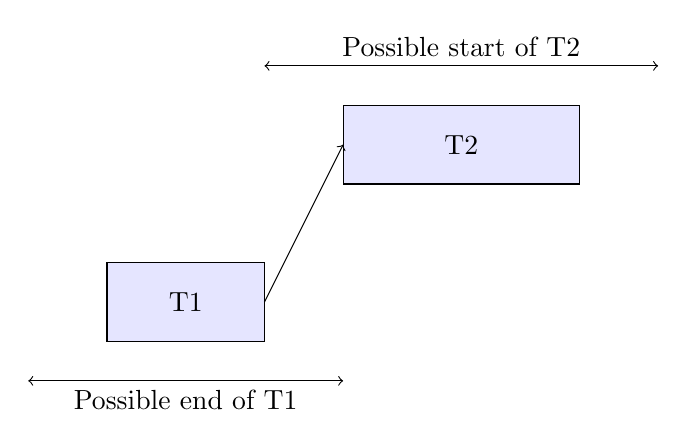
\begin{tikzpicture}
\draw[fill=blue!10,draw=black] (0,0) rectangle node {T1} (2,1);
\draw[fill=blue!10,draw=black] (3,2) rectangle node {T2} (6,3);
\draw[->] (2,0.5) -- (3,2.5);
\draw[<->] (2,3.5) -- node[above] {Possible start of T2}(7,3.5);
\draw[<->] (-1,-0.5) -- node[below] {Possible end of T1}(3,-0.5);
\end{tikzpicture}
}
\end{column}
\end{columns}
\end{frame}

\begin{frame}
\frametitle{Less Common: startBeforeStart}
\begin{columns}
\begin{column}{0.5\textwidth}
\begin{itemize}
\item States that one task (T2) can start any time after the start of another task (T1)
\item Uncommon in manufacturing, occurs in project management
\item Example later on on assembly line balancing 
\end{itemize}
\end{column}
\begin{column}{0.5\textwidth}
\scalebox{0.6}{
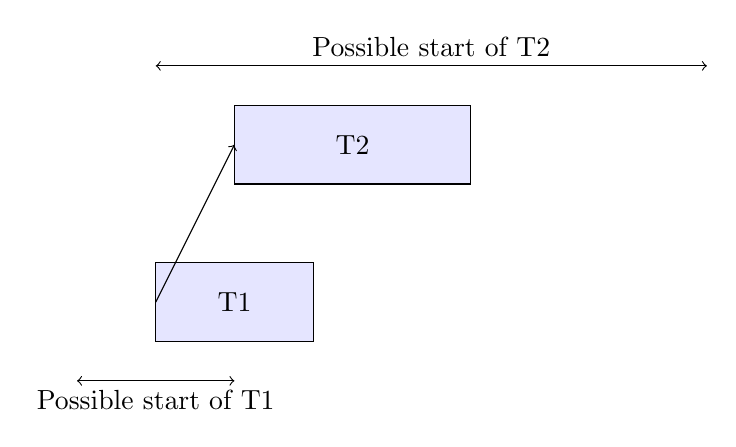
\begin{tikzpicture}
\draw[fill=blue!10,draw=black] (0,0) rectangle node {T1} (2,1);
\draw[fill=blue!10,draw=black] (1,2) rectangle node {T2} (4,3);
\draw[->] (0,0.5) -- (1,2.5);
\draw[<->] (0,3.5) -- node[above] {Possible start of T2}(7,3.5);
\draw[<->] (-1,-0.5) -- node[below] {Possible start of T1}(1,-0.5);
\end{tikzpicture}
}
\end{column}
\end{columns}
\end{frame}

\begin{frame}
\frametitle{NoWait}
\begin{columns}
\begin{column}{0.5\textwidth}
\begin{itemize}
\item Sometimes, two steps must follow each other immediately
\item The item made would spoil
\item Product specific
\item There is no space to hold item
\item Machine specific, buffers
\item End of one task (T1) must be equal to start of next task (T2)
\item May mean delay of start of task T1
\end{itemize}
\end{column}
\begin{column}{0.5\textwidth}
\input{../02-concepts/nowait}
\end{column}
\end{columns}
\end{frame}

\begin{frame}
\frametitle{Blocking}
\begin{columns}
\begin{column}{0.5\textwidth}
\begin{itemize}
\item Sometimes, two steps must follow each other immediately
\item There is no space to hold store item between machines
\item Keep item on previous machine until needed
\item That machine is now blocked
\item Duration of task T1 is extended
\item Use with caution!
\end{itemize}
\end{column}
\begin{column}{0.5\textwidth}
\scalebox{0.6}{
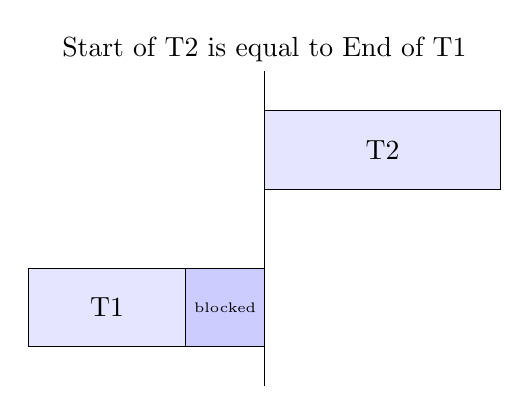
\begin{tikzpicture}
\draw[fill=blue!10,draw=black] (0,0) rectangle node {T1} (2,1);
\draw[fill=blue!20,draw=black] (2,0) rectangle node {\tiny blocked} (3,1);
\draw[fill=blue!10,draw=black] (3,2) rectangle node {T2} (6,3);
\draw[] (3,-0.5) -- (3,3.5) node[above] {Start of T2 is equal to End of T1};
\end{tikzpicture}
}
\end{column}
\end{columns}
\end{frame}


\begin{frame}
\frametitle{More General: Relations between Intervals}
\begin{columns}
\begin{column}{0.5\textwidth}
\begin{itemize}
\item First introduced by Allen (1983)
\item 13 relations between intervals
\item Allows composition of relations
\item Constraint reasoning on sets of relations
\end{itemize}
\end{column}
\begin{column}{0.5\textwidth}
\includegraphics[width=\textwidth]{../02-concepts/images/allen-relations}

{\tiny from Wikipedia: \url{https://en.wikipedia.org/wiki/Allen\%27s_interval_algebra}}
\end{column}
\end{columns}
\end{frame}


\subsection{Relation between Tasks and Jobs}



\subsection{Jobs: Release and Due Date}

\section{Processes, Bill of Materials}

\section{Problem Classification}

\subsection{Job-Shop}
\subsection{Flow-Shop}
\subsection{Open-Shop}
\subsection{RCPSP}
\subsection{$\alpha$, $\beta$, $\gamma$ Notation}

\section{Key Visualization Methods}

\section{Summary}

\begin{frame}
\frametitle{Summary}
\begin{itemize}
\item We introduced the key concepts for scheduling problems
\item Orders, products, processes
\item Jobs and tasks
\item Existing problem classifications
\begin{itemize}
\item Academic
\item Limited practical usefulness
\end{itemize}
\item Key visualization methods
\end{itemize}
\end{frame}

